\documentclass[tikz,border=6pt]{standalone}
\usepackage{fontspec}
\setmainfont{Noto Sans}
\usepackage{amsmath}
\usepackage{tikz}
\usetikzlibrary{arrows.meta,positioning,calc}
\definecolor{cudaG}{RGB}{118,185,0}
\definecolor{sadRed}{RGB}{200,60,50}
\definecolor{gray5}{RGB}{85,85,85}
\begin{document}
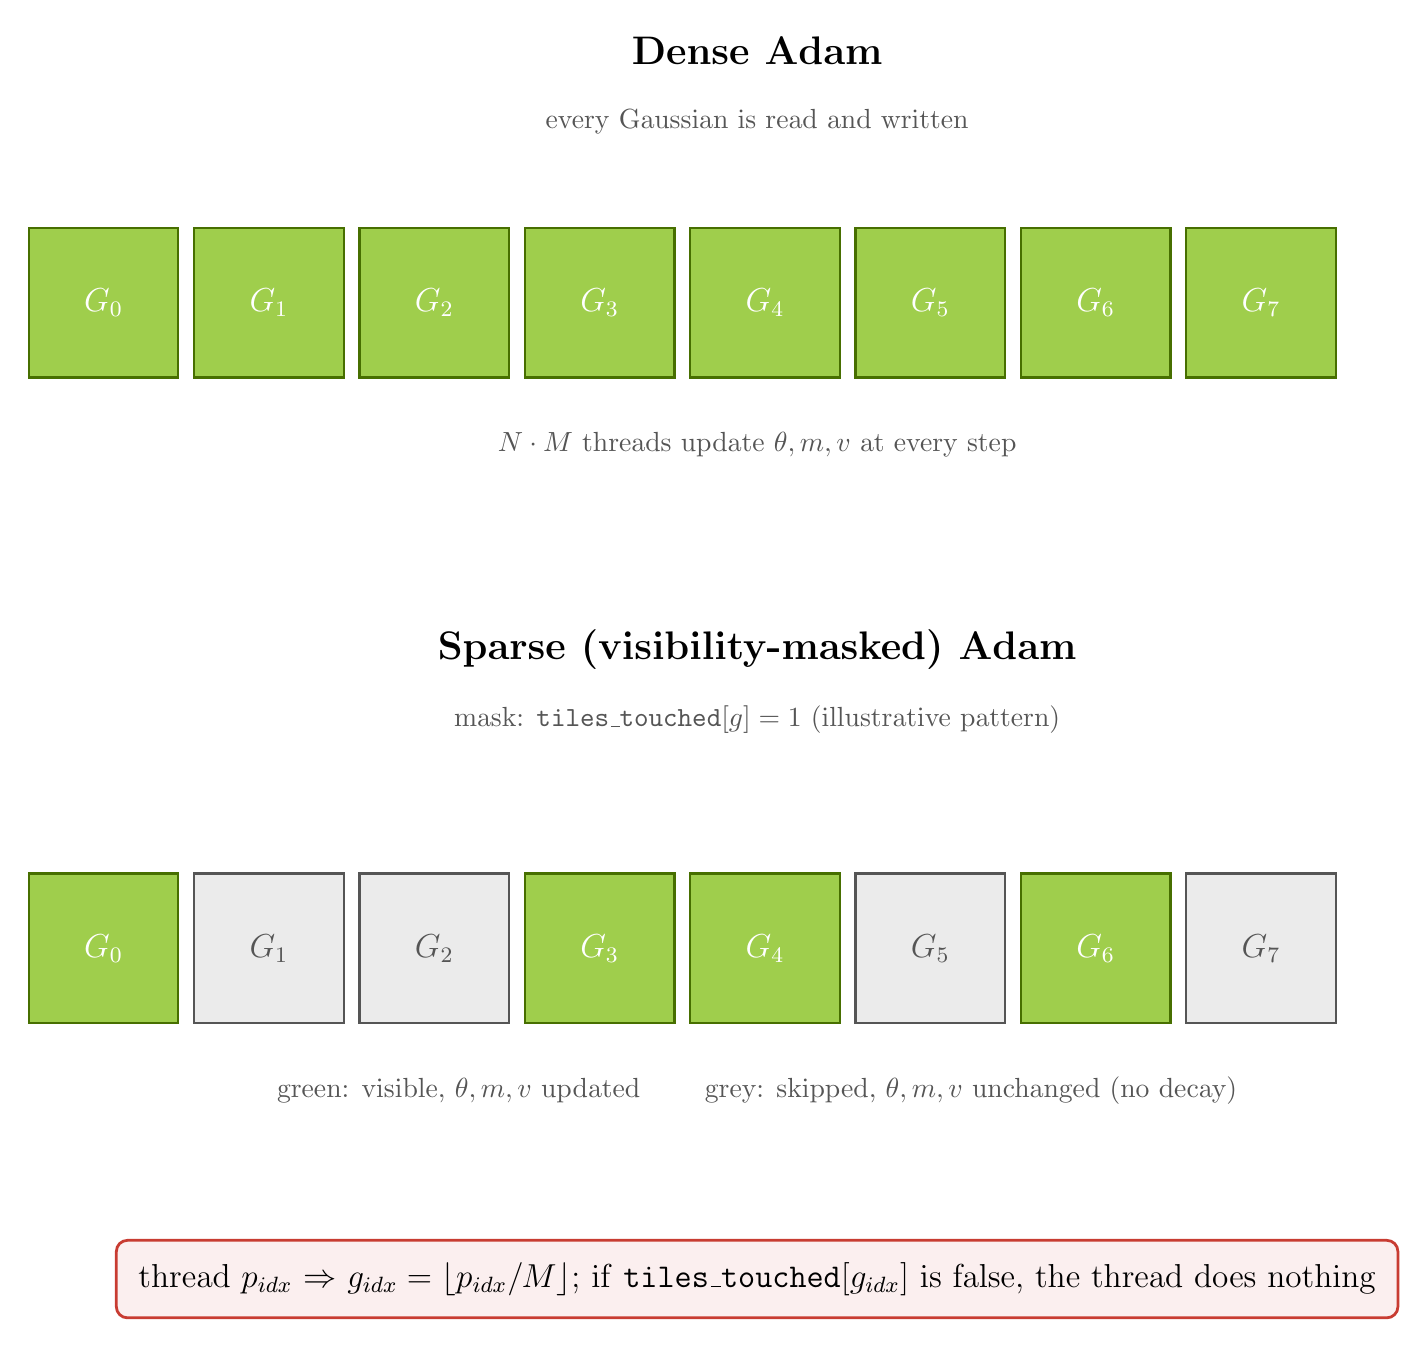
\begin{tikzpicture}[
  >=Stealth,
  g/.style={draw=gray5,line width=0.8pt,minimum width=1.9cm,minimum height=1.9cm,font=\large,align=center},
  on/.style={g,fill=cudaG!70,draw=cudaG!60!black,text=white},
  off/.style={g,fill=gray5!12,draw=gray5,text=gray5},
  lab/.style={font=\Large\bfseries,align=center}
]
  % Dense panel
  \node[lab] at (8.3,3.2) {Dense Adam};
  \node[font=\normalsize,gray5] at (8.3,2.3) {every Gaussian is read and written};
  \foreach \i in {0,...,7} {
    \node[on] at (\i*2.1,0) {$G_{\i}$};
  }
  \node[font=\normalsize,gray5,align=center] at (8.3,-1.8) {$N \cdot M$ threads update $\theta,m,v$ at every step};

  % Sparse panel
  \node[lab] at (8.3,-4.4) {Sparse (visibility-masked) Adam};
  \node[font=\normalsize,gray5] at (8.3,-5.3) {mask: \texttt{tiles\_touched}$[g]=1$ (illustrative pattern)};
  \foreach \i/\vis in {0/1,1/0,2/0,3/1,4/1,5/0,6/1,7/0} {
    \ifnum\vis=1
      \node[on] at (\i*2.1,-8.2) {$G_{\i}$};
    \else
      \node[off] at (\i*2.1,-8.2) {$G_{\i}$};
    \fi
  }
  \node[font=\normalsize,align=center,gray5] at (8.3,-10.0) {green: visible, $\theta,m,v$ updated \qquad grey: skipped, $\theta,m,v$ unchanged (no decay)};

  % Formula
  \node[draw=sadRed,line width=1pt,rounded corners,fill=sadRed!8,font=\large,inner sep=8pt,align=center] at (8.3,-12.4)
    {thread $p_{idx}$ $\Rightarrow$ $g_{idx}=\lfloor p_{idx}/M\rfloor$; if \texttt{tiles\_touched}$[g_{idx}]$ is false, the thread does nothing};
\end{tikzpicture}
\end{document}
